\section{RESULTADOS E DISCUSSÃO}
  A coleta ocorreu em 26 de junho de 2025, das 08:05 às 08:14 (horário local, America/Porto\_Velho). Em 9 minutos foram registrados 6 tentativas de login voluntárias de estudantes. Após a coleta, os dados foram exportados para CSV e processados para análise estatística e visualização.

  \subsection{Padrões Observados}
    Alguns padrões foram identificados a partir dos dados coletados durante o experimento, incluindo perfil de dispositivos, navegadores, sistemas operacionais, classificação entre plataformas móveis e desktop, além da distribuição temporal dos acessos.

    \subsection{Perfil de Dispositivos}
    No perfil de dispositivos (Figura~\ref{fig:devices}), observa-se uma distribuição equilibrada entre estações de trabalho e dispositivos móveis. Desktops com Windows 10/11 e macOS representaram metade dos acessos, enquanto smartphones Android (Samsung A52 e Motorola G53) e iOS (iPhone) corresponderam à outra metade. Esse balanceamento indica que tanto usuários em ambiente fixo quanto em trânsito interagiram de forma semelhante com o portal falso, sugerindo que estratégias de conscientização devem contemplar ambos os cenários para maximizar o alcance das campanhas de segurança.

    \begin{figure}[H]
    \centering
        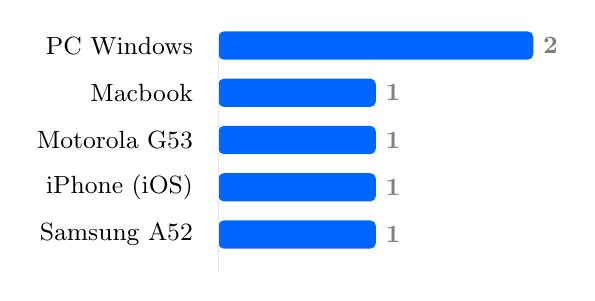
\begin{tikzpicture}[yscale=0.6]
        % Dados: valor/{Nome do Dispositivo}
        \foreach \val/\name [count=\i] in {2/{PC Windows}, 1/{Macbook}, 1/{Motorola G53}, 1/{iPhone (iOS)}, 1/{Samsung A52}} {
            \fill[blue!60!cyan, rounded corners=2pt] (0,-\i) rectangle (\val*2, -\i+0.6);
            \node[left, font=\small] at (-0.2, -\i+0.3) {\name};
            \node[right, font=\small\bfseries, gray] at (\val*2, -\i+0.3) {\val};
        }
        % Linha lateral discreta
        \draw[gray!20] (0,-0.5) -- (0,-5.5);
    \end{tikzpicture}
    \caption{Distribuição de dispositivos.}
     \label{fig:devices}
\end{figure}



    Observa-se que 50\% dos acessos partiram de desktops (Windows/macOS) e 50\% de dispositivos móveis (Android/iOS), indicando uso equilibrado entre perfis fixo e portátil.

\subsubsection{Perfil de Navegadores}
\begin{figure}[H]
    \centering
    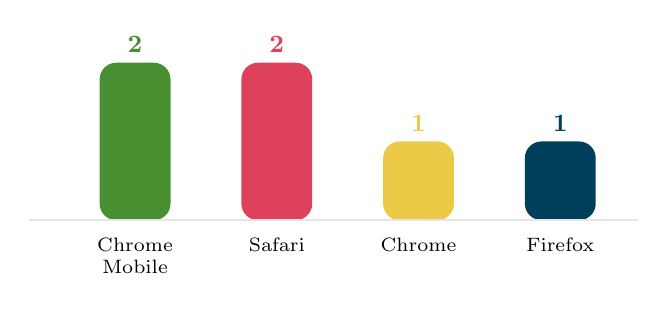
\begin{tikzpicture}[xscale=1.8]
        % Paleta de cores modernas
        \definecolor{color1}{HTML}{488f31}
        \definecolor{color2}{HTML}{de425b}
        \definecolor{color3}{HTML}{edc948}
        \definecolor{color4}{HTML}{003f5c}
    
        % Dados: {valor/rótulo/cor}
        \foreach \val/\name/\c [count=\i] in {2/{Chrome\\Mobile}/color1, 2/{Safari}/color2, 1/{Chrome}/color3, 1/{Firefox}/color4} {
            
            % Barra estilo pílula (Ponta arredondada)
            \fill[\c, rounded corners=6pt] (\i,0) rectangle (\i+0.5, \val);
            
            % Valor acima da barra
            \node[above, font=\small\bfseries, \c] at (\i+0.25, \val) {\val};
            
            % Rótulo abaixo (com quebra de linha se necessário)
            \node[below, font=\scriptsize, align=center] at (\i+0.25, -0.1) {\name};
        }
        
        % Linha de base decorativa
        \draw[gray!20, thick] (0.5,0) -- (4.8,0);
    \end{tikzpicture}
    \caption{Distribuição dos navegadores.}
\end{figure}

    A família Chrome (mobile + desktop) responde por 50\% dos acessos, seguida por Safari (33\%) e Firefox (17\%), evidenciando dependência de engines Chromium e WebKit.

\subsubsection{Distribuição por Sistema Operacional}
\begin{figure}[H]
  \centering
  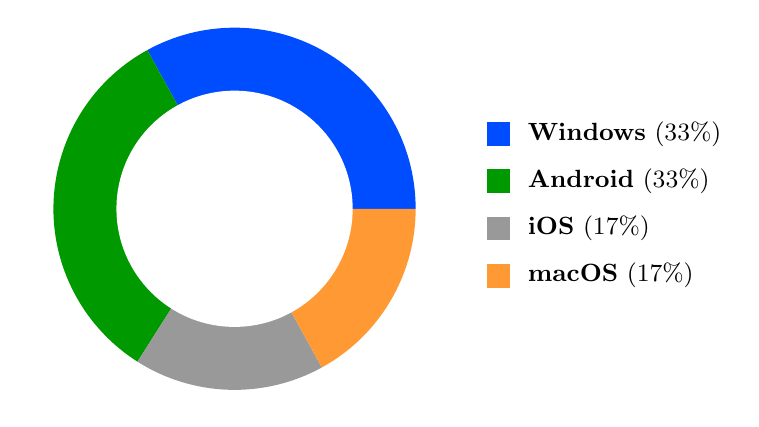
\begin{tikzpicture}
    % Fatias (Donut) usando cores padrão do TikZ/LaTeX
    % Windows - 33% (0 a 118.8 graus)
    \fill[blue!70!cyan] (0,0) -- (0:2.3) arc (0:118.8:2.3) -- cycle;
    % Android - 33% (118.8 a 237.6 graus)
    \fill[green!60!black] (0,0) -- (118.8:2.3) arc (118.8:237.6:2.3) -- cycle;
    % iOS - 17% (237.6 a 298.8 graus)
    \fill[black!40] (0,0) -- (237.6:2.3) arc (237.6:298.8:2.3) -- cycle;
    % macOS - 17% (298.8 a 360 graus)
    \fill[orange!80] (0,0) -- (298.8:2.3) arc (298.8:360:2.3) -- cycle;

    % Buraco central (efeito Donut)
    \fill[white] (0,0) circle (1.5);

    % Legenda Lateral Organizada
    \begin{scope}[shift={(3.2, 0.8)}]
      \fill[blue!70!cyan] (0,0) rectangle (0.3,0.3) node[right, black] at (0.4, 0.15) {\small \textbf{Windows} (33\%)};
      \fill[green!60!black] (0,-0.6) rectangle (0.3,-0.3) node[right, black] at (0.4, -0.45) {\small \textbf{Android} (33\%)};
      \fill[black!40] (0,-1.2) rectangle (0.3,-0.9) node[right, black] at (0.4, -1.05) {\small \textbf{iOS} (17\%)};
      \fill[orange!80] (0,-1.8) rectangle (0.3,-1.5) node[right, black] at (0.4, -1.65) {\small \textbf{macOS} (17\%)};
    \end{scope}
  \end{tikzpicture}
  \caption{Proporção de sistemas operacionais.}
\end{figure}

    Windows e Android lideram com 33\% cada, reforçando a predominância de plataformas da Microsoft e Google.

\subsubsection{Classificação Mobile vs Desktop}
\begin{figure}[H]
  \centering
  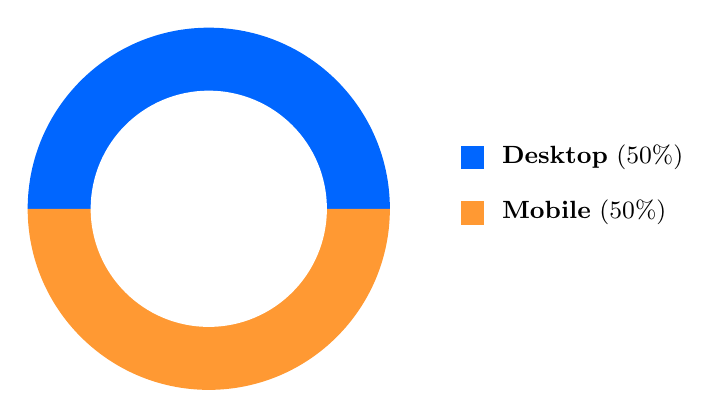
\begin{tikzpicture}
    % Fatias (Donut) - 50% cada (180 graus)
    % Desktop - Azul
    \fill[blue!60!cyan] (0,0) -- (0:2.3) arc (0:180:2.3) -- cycle;
    % Mobile - Laranja/Âmbar
    \fill[orange!80] (0,0) -- (180:2.3) arc (180:360:2.3) -- cycle;

    % Buraco central (efeito Donut)
    \fill[white] (0,0) circle (1.5);

    % Legenda Lateral Organizada
    \begin{scope}[shift={(3.2, 0.5)}]
      \fill[blue!60!cyan] (0,0) rectangle (0.3,0.3) 
        node[right, black] at (0.4, 0.15) {\small \textbf{Desktop} (50\%)};
      
      \fill[orange!80] (0,-0.7) rectangle (0.3,-0.4) 
        node[right, black] at (0.4, -0.55) {\small \textbf{Mobile} (50\%)};
    \end{scope}
  \end{tikzpicture}
  \caption{Acessos: mobile vs desktop.}
\end{figure}

   Meio a meio entre mobile e desktop, sugerindo que estratégias de conscientização devem abranger ambos os perfis.

\subsubsection{Distribuição Temporal dos Acessos}
\begin{figure}[H]
  \centering
  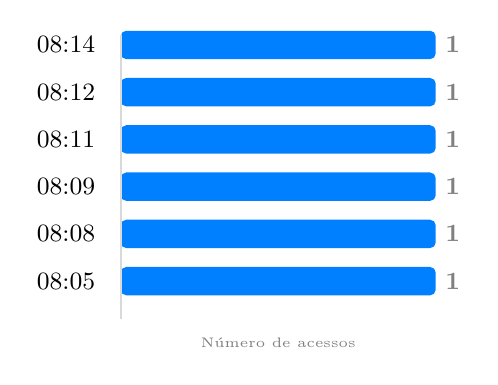
\begin{tikzpicture}[yscale=0.6]
    % Dados: valor/{Horário}
    \foreach \val/\name [count=\i] in {1/{08:14}, 1/{08:12}, 1/{08:11}, 1/{08:09}, 1/{08:08}, 1/{08:05}} {
        
        % Barras horizontais (valor * 4 para dar largura, já que todos são 1)
        \fill[blue!50!cyan, rounded corners=2pt] (0,-\i) rectangle (\val*4, -\i+0.6);
        
        % Horários à esquerda
        \node[left, font=\small] at (-0.2, -\i+0.3) {\name};
        
        % Valor numérico ao final da barra
        \node[right, font=\small\bfseries, gray] at (\val*4, -\i+0.3) {\val};
    }
    % Linha de base vertical sutil
    \draw[gray!30, thick] (0,-0.5) -- (0,-6.5);
    
    % Rótulo do eixo X (opcional, para clareza)
    \node[font=\tiny, gray] at (2, -7) {Número de acessos};
  \end{tikzpicture}
  \caption{Acessos por minuto entre 08:05 e 08:14.}
\end{figure}

 Os acessos se distribuíram de forma uniforme ao longo dos 9 minutos de atividade, sem concentração em um único instante.

 \subsection{Análise de Padrões}
    \begin{itemize}
      \item \textbf{Uso corporativo de Chrome:} A prevalência do Chrome sugere necessidade de avaliar configurações de WebView em apps acadêmicos.
      \item \textbf{Equilíbrio mobile/desktop:} Campanhas de conscientização devem abordar usuários de ambas as plataformas.
      \item \textbf{Acessos pontuais:} Ausência de picos indica participação voluntária homogênea, sem efeito de “manada”.
    \end{itemize}